\documentclass[11pt]{article}

\usepackage[UTF8]{ctex}

\usepackage[T1]{fontenc}

\usepackage[utf8]{inputenc}

\usepackage{lmodern}

\usepackage{amsmath}

\usepackage{amssymb}

\usepackage{booktabs}
\usepackage{longtable}
% Shared presentation for every main-text and supplementary table.
% Keep small-size superscripts legible and use the same math fonts throughout.
\DeclareMathSizes{10}{10}{8}{6}
\newcommand{\papertablestyle}{%
    \small
    \setlength{\tabcolsep}{3.5pt}%
    \renewcommand{\arraystretch}{1.22}%
    \setlength{\heavyrulewidth}{0.7pt}%
    \setlength{\lightrulewidth}{0.4pt}%
    \setlength{\cmidrulewidth}{0.3pt}%
    \setlength{\defaultaddspace}{3pt}%
    \setlength{\abovetopsep}{4pt}%
    \setlength{\abovecaptionskip}{6pt}%
    \setlength{\belowcaptionskip}{6pt}%
}
\newcommand{\papertablehead}[2]{\shortstack[c]{#1\\#2}}


\usepackage{graphicx}

\usepackage{placeins}

\setcounter{topnumber}{3}
\setcounter{totalnumber}{4}
\renewcommand{\topfraction}{0.9}
\renewcommand{\textfraction}{0.1}
\renewcommand{\floatpagefraction}{0.7}
\setlength{\textfloatsep}{12pt plus 2pt minus 2pt}
\setlength{\floatsep}{10pt plus 2pt minus 2pt}
\setlength{\intextsep}{10pt plus 2pt minus 2pt}
\makeatletter
\newenvironment{inlinefigure}
  {\par\addvspace{\intextsep}\noindent\begin{minipage}{\linewidth}\def\@captype{figure}\centering}
  {\end{minipage}\par\addvspace{\intextsep}}
\makeatother

\usepackage[margin=1in]{geometry}

\usepackage[hidelinks]{hyperref}



\graphicspath{{../figures/}}

\newcommand{\tablepath}{../tables}




\setlength{\emergencystretch}{1.5em}

\title{有限输入等待下的非侵入式语言解码：局部上下文与滚动修正}
\author{}
\date{}

\begin{document}
\maketitle
\nocite{moses2021neuroprosthesis,willett2023speech,card2024speech,wairagkar2025voice,defossez2023decoding,dascoli2025word,levy2026brain2qwerty,littlejohn2025streaming,lu2025braininspired,jayalath2025unlocking}
% !TeX root = main.tex

\renewcommand{\abstractname}{摘要}
\begin{abstract}
在非侵入式词级语言解码中，联合建模邻近词窗可提高预测性能，但依赖目标词之后的输入也会增加输出等待。
本文面向已知词级对齐的自然连续语音聆听任务，提出一种有限输入等待下的局部上下文与滚动修正方法，
使同一词位能够先输出初判，再随最多两个后续词窗到达逐步更新，并固定更早的预测。
实验采用法语脑磁（Pallier2025）和中文脑电（ChineseEEG-2）数据。
在固定 $50$ 词候选集上，半径为 $2$ 的局部上下文相较完整上下文模型，
宏平均 Top-$10$ 分别提高 $5.10$ 和 $5.12$ 个百分点；
共享滚动模型从 K0 更新至 K2 时，该指标分别提高 $19.06$ 和 $14.53$ 个百分点。
序列解码以法语 MEG 为主要分析场景：滚动策略使平均片段 BLEU-1 从 $8.37\%$ 提高至 $13.46\%$，
而固定初始表示的文本重搜仅产生较小改善。
中文 EEG 上的文本收益主要体现于 WER 和词位准确率。
滚动策略相对首次预测平均增加约半秒的神经输入等待，比完整片段策略平均减少约 $1.5$--$1.8$ 秒。
上述结果表明，有限回修可在既定词级对齐与序列搜索协议下提供质量—等待折中。
\end{abstract}

\section{引言}

从脑活动中恢复语言是脑机接口研究的重要目标。
侵入式接口已经能够实现大词汇文本解码和接近实时的语音合成
\cite{moses2021neuroprosthesis,willett2023speech,card2024speech,wairagkar2025voice}。
EEG 和 MEG 无需手术植入，但信号较弱。
借助预训练语音和语言模型，非侵入式解码已从连续语音片段检索推进到词级解码
\cite{defossez2023decoding,dascoli2025word}，
其中联合建模相邻词的神经表示可以显著改善预测\cite{dascoli2025word}。

联合建模目标词之后的神经活动，会将解码质量与输入等待耦合在一起。
本文在法语 MEG（Pallier2025）和中文 EEG（ChineseEEG-2）两个自然语音聆听数据集上，
考察词级解码需要多大范围的神经上下文，以及后续输入能否在有限等待下修正已有预测。
目标词左右各最多两个词的局部窗口在宏平均 Top-$10$ 上优于完整上下文模型；
据此，我们让目标词在自身神经窗可用后先给出预测，再随少量后续词窗到达逐步更新，更早的输出依次固定。
贡献如下：
\begin{itemize}
    \item 比较局部词窗与完整上下文在法语 MEG 和中文 EEG 两个自然连续聆听数据条件下的词级检索表现，
          考察较小上下文范围是否足以达到良好的候选排序性能。
    \item 提出共享参数的滚动修正策略，在最多两个后续词窗可用时更新历史词位预测，
          并设置固定 K0 表示的重搜策略，分析表示更新与近期文本搜索的共同作用。
    \item 在词级及序列级评价中考察有限输入等待下的预测质量、回修收益和输出稳定性；
          主要报告法语 MEG 的序列解码比较，并在中文 EEG 上检验相同协议的表现。
\end{itemize}

\section{相关工作}

\subsection{非侵入式词级解码与神经上下文}

Défossez 等人通过对比学习将 EEG/MEG 与预训练语音表示对齐，
在自然连续语音条件下实现了语音片段检索\cite{defossez2023decoding}。
d'Ascoli 等人进一步将词级神经活动映射到语言表示空间，
并利用跨词上下文提高单词检索性能\cite{dascoli2025word}。
Brain2Qwerty 在打字句子解码中先提取局部神经特征，
再建模字符之间的关系，并结合语言模型改善文本\cite{levy2026brain2qwerty}。
这些工作表明，目标之外的序列上下文有助于预测，
但对上下文范围与输入可用时刻的联合比较仍较有限。
SimpleB2T 进一步指出，词对齐的重叠窗口可能提供词间时间线索\cite{jayalath2026timing}。
本文不试图识别跨词性能提升的具体神经机制，而是在已知词级对齐的既定条件下，
比较局部上下文范围及其对应的输入等待，并研究有限范围内的连续预测修正。

\subsection{增量神经解码}

侵入式语言脑机接口中，随神经信号到达而更新输出已有较多研究。
Moses 等人在新的词级证据出现后结合语言模型调整此前的文本假设
\cite{moses2021neuroprosthesis}；
Willett 等人持续更新音素概率并进行语言模型搜索，实现流式文本解码
\cite{willett2023speech}；
脑到语音系统则将更新间隔进一步缩短\cite{littlejohn2025streaming}。
文本搜索可以随着新证据到达改变历史假设。
本文关注目标神经表示的更新：后续神经活动直接参与较早目标的表示计算，
使同一目标在获得更多输入后产生新的候选分布。
非侵入式方面，CogReader 将 fMRI 序列分段，
把已解码内容的语义表示传递给后续片段\cite{lu2025braininspired}，
主要利用历史辅助未来预测。

\subsection{同步机器翻译与流式输出}

在输入等待与质量之间取舍，是同步机器翻译和流式语音识别中的核心问题。
wait-$k$ 策略先读入 $k$ 个源词，再交替读入与输出，使目标生成保持固定的源端词数滞后
\cite{ma2019stacl}。
重翻译方法允许修改已输出的内容，并用归一化擦除指标衡量显示稳定性
\cite{arivazhagan2020retranslation}。
本文同样限制需要等待的后续输入，并允许近期预测继续修正：
先依据当前输入给出预测，再在至多两个后续词窗内更新目标神经表示与文本，随后固定。

% !TeX root = main.tex

\section{方法}

\subsection{问题定义}

给定包含 $n$ 个连续词的语言片段 $w_1,\ldots,w_n$，
词级神经编码器将第 $i$ 个词对应的 EEG/\allowbreak{}MEG 窗编码为神经表示 $\mathbf z_i$。
上下文模型联合建模若干相邻的 $\mathbf z$，
取目标位置的输出与冻结的文本表示对齐，得到目标词的候选排序；
文本序列解码再结合语言评分，将各词位的候选组织为连续文本。

实验按词窗的时间顺序重放离线数据，仅使用当前已经获得的神经输入。
词级对齐、片段边界和词数视为已知。


\subsection{局部神经上下文}

对目标位置 $i$，取其左侧 $l$ 个和右侧 $r$ 个相邻词，构成局部上下文
\[
\mathbf{Z}_i^{(l,r)}
=(\mathbf{z}_{i-l},\ldots,\mathbf{z}_i,\ldots,\mathbf{z}_{i+r}),
\]
索引在片段边界处截断至 $[1,n]$。
该序列输入上下文 Transformer 模型 $f_{\mathrm{ctx}}$，只取目标位置 $i$ 对应的输出隐状态并经 $L_2$ 归一化，得到上下文神经表示：
\[
\hat{\mathbf{y}}_i^{(r)} = \frac{f_{\mathrm{ctx}}(\mathbf{Z}_i^{(l,r)})_i}{\|f_{\mathrm{ctx}}(\mathbf{Z}_i^{(l,r)})_i\|_2} .
\]
令 $l=r=k$ 即得到半径为 $k$ 的对称窗口，改变 $k$ 可以考察检索性能对上下文范围的依赖。
右侧范围 $r$ 同时决定了目标词需要等待多少后续输入。


\subsection{滚动修正}

每个词的神经窗取其语音起点后 $1\,\mathrm{s}$ 的信号；
下文称某个词窗“到达”，指该窗已完整可用。
目标词 $i$ 的词窗到达时，模型以 $\mathbf Z_i^{(k,0)}$ 给出首次预测；
此后每到达一个后续词窗，就以扩展后的 $\mathbf Z_i^{(k,r)}$ 重新预测，直至 $r=R$：
\[
\hat{w}_i^{(0)}\rightarrow\hat{w}_i^{(1)}\rightarrow\cdots\rightarrow\hat{w}_i^{(R)}.
\]
本文取 $k=R=2$，并将三个可见状态记为
\[
\mathrm{K0}:[-2,0],\qquad\mathrm{K1}:[-2,1],\qquad\mathrm{K2}:[-2,2].
\]
第 $t$ 个词窗到达时，模型给出词 $t$ 的 K0 预测，
同时将词 $t-1$ 和 $t-2$ 分别更新到 K1 和 K2；
可修正区域随 $t$ 向前滚动（图~\ref{fig:rolling_revision_method}）。
片段边界处只使用片段内实际存在的词窗。

\begin{figure}[!htbp]
    \centering
    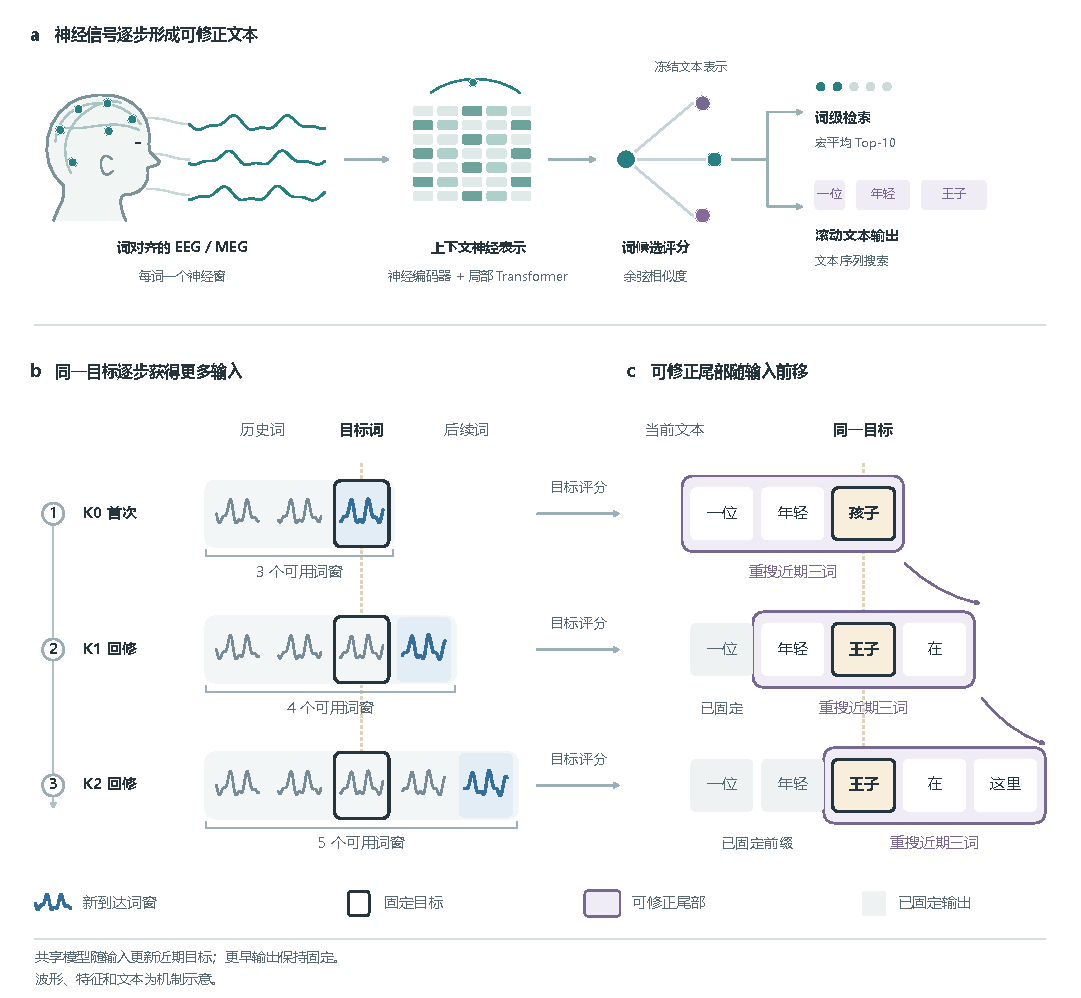
\includegraphics[width=\linewidth]{method_overview_editorial.pdf}
    \caption{滚动修正示意。蓝色为新到达的神经窗，黑框为固定目标，紫色为近期可回修词位，灰色为已固定输出。共享模型随新词窗到达更新近期表示并重新搜索文本。}
    \label{fig:rolling_revision_method}
\end{figure}

\subsection{输入等待}
\label{sec:input_wait}

设词 $i$ 的语音起点为 $\tau_i$，神经窗长度为 $T=1\,\mathrm{s}$。
若目标词最多等待 $R$ 个后续词窗，其最终预测所需输入的可用时刻为
\[
c_i^{(R)}=\tau_{\min(i+R,\,n)}+T .
\]
$R=0$ 对应首次预测，$R\ge n-i$ 对应等待片段末词窗的完整片段解码。
本文报告的总输入等待为 $c_i^{(R)}-\tau_i$。
输入等待按神经输入的可用时间计算，不含模型推断与文本搜索开销。


\subsection{共享滚动训练}
\label{sec:revision_training}

训练分两个阶段。
先训练不含跨词上下文的词模型；
再用其初始化神经编码器，新建上下文模型进行滚动训练。
K0、K1 和 K2 共享同一组参数。

滚动训练按词窗到达顺序模拟预测过程：
第 $t$ 个词窗到达时，同时监督词 $t$ 的 K0、词 $t-1$ 的 K1 和词 $t-2$ 的 K2 预测，
片段边界处不存在的状态跳过。
设批次 $b$ 中含有效目标的状态集合为 $D_b$，
各状态先在其目标上平均对比损失，再等权平均：
\[
\mathcal{L}_b
=\frac{1}{|D_b|}\sum_{r\in D_b}\mathcal{L}_b^{(r)} .
\]
对比负样本取批次内的其他文本目标，并屏蔽与目标相同的词。


\subsection{文本序列解码}
\label{sec:sentence_decoding_method}

参考 \cite{jayalath2025unlocking}，我们将神经候选与语言模型评分结合，
在已知词数的条件下逐词进行束搜索。
每个词位的候选包括两部分：
训练词库 $V$ 中神经相似度最高的若干词，以及语言模型根据当前前缀 $u$ 提出的续写词。
后者可以位于 $V$ 之外，同样由冻结文本编码器获得表示。

在可见状态 $r$ 下，目标位置 $i$ 的归一化神经表示 $\hat{\mathbf y}_i^{(r)}$
与候选词表示 $\mathbf y(w)$ 的余弦相似度经缩放后，
在 $V$ 及当前提出的词库外候选上做 softmax 归一化，得到神经概率 $p_{\mathrm N}$。
候选词的得分为
\[
s_i^{(r)}(w\mid u)
=\log p_{\mathrm N}(w\mid\hat{\mathbf y}_i^{(r)},u)
+\lambda\ell_{\mathrm{LM}}(w\mid u),
\]
其中 $\lambda$ 为语言评分权重，$\ell_{\mathrm{LM}}$ 为加入候选词前后整串文本的对数概率之差。
束搜索逐词累加得分，具体参数见附录~\ref{sec:supp_sentence_settings}。

在此基础上比较表~\ref{tab:strategies} 中的六种策略。
近期重搜保持更早的前缀固定，策略 F 从空前缀开始搜索整个片段。
F-local 与 F 使用相同的完整片段输入等待和整段搜索，
但复用 C 的最终局部表示：内部词位为 K2，末两个词位按片段边界使用 K1 和 K0。
B 用于区分神经表示更新与文本重搜的作用，新词仍以其自身 K0 表示进入搜索。
各策略使用相同的候选构造、语言评分和搜索参数。

\begin{table}[!htbp]
    \centering
    \papertablestyle
    \caption{文本序列解码策略。}
    \label{tab:strategies}
    % Definitions of the six frozen text-decoding strategies; no experimental results.
\begingroup
\papertablestyle
\begin{tabular}{@{}llccc@{}}
\toprule
策略 & 名称 & 神经表示 & 每次重搜词位 & 输出固定时刻 \\
\midrule
A  & 固定输出     & K0                       & 1（当前词） & $c_i^{(0)}$ \\
B  & 固定表示重搜 & K0                       & 3           & $c_i^{(2)}$ \\
C1 & 一次回修     & K0$\to$K1                & 2           & $c_i^{(1)}$ \\
C  & 滚动修正     & K0$\to$K1$\to$K2         & 3           & $c_i^{(2)}$ \\
F  & 完整片段     & 完整上下文               & 整段        & $\tau_n+T$ \\
F-local & 局部整段 & K2                       & 整段        & $\tau_n+T$ \\
\bottomrule
\end{tabular}
\endgroup

\end{table}

\section{实验设置}

\subsection{数据集}

我们在两个自然连续语音聆听数据集上进行实验：法语 MEG 数据集 Pallier2025 和中文 EEG 数据集 ChineseEEG-2，两者的刺激材料均为《小王子》有声书。
训练、验证和测试集按语言篇章划分，所有受试者使用相同划分，测试集篇章在模型训练中完全未见。

ChineseEEG-2\cite{chen2026chineseeeg2} 使用 Passive Listening 条件下 8 名受试者的 128 通道 EEG。
由于实际朗读与原文之间存在停顿、漏读、增读或替换，
我们依据实际播放音频重新核对了词级内容和时间戳。
中文使用 jieba 精确模式分词，关闭 HMM 新词识别；
英文和阿拉伯数字保留原文本组，标点不作为带时间戳的词事件。
第 3、5、25 章用于验证，第 2、9 章用于测试，其余有效章节用于训练。

Pallier2025\cite{openneuro_pallier2025_listening,dascoli2025word} 使用 10 名受试者的 306 个 MEG 传感器（102 个磁强计、204 个平面梯度计），
以 listening run 为划分单位：run-07 用于验证，run-06 用于测试，其余有效 run 用于训练。

有官方预处理结果的数据直接使用该结果，所有信号统一重采样至 $50$~Hz。


\subsection{模型与训练}

本文以 d'Ascoli 等人的词级解码框架为基础\cite{dascoli2025word}。
文本目标由冻结的 BGE-M3 编码器\cite{chen2024bgem3} 得到：每个词单独编码，
取末层首个 token 的 $1024$ 维隐藏状态，并做 $L_2$ 归一化。
训练词库只包含训练材料中的词。

神经端以每个词语音起点后 $1\,\mathrm{s}$ 的信号为输入，
经基于传感器位置的通道映射和残差膨胀卷积网络得到 $\mathbf z_i$，
上下文模型为 Transformer。
训练按第~\ref{sec:revision_training}~节的两阶段进行，
每个数据集使用三个随机种子。
网络结构与超参数见附录表~\ref{tab:model_settings}。

上下文范围实验比较半径 $k\in\{0,1,2,4,8\}$ 的对称窗口，
以及使用片段内全部词的完整上下文模型。
各条件均包含上下文 Transformer，半径 $0$ 即只输入目标词。
可见状态实验固定两个历史词，
将共享滚动模型的三个状态与分别训练的 $[-2,r]$ 模型（$r=0,1,2$）进行比较。
验证集上，对称窗口的平均宏平均 Top-$10$ 在 Pallier2025 中以 $k=2$ 最高，
在 ChineseEEG-2 中以 $k=4$ 最高。
结合局部窗口的验证结果，滚动模型统一取两个历史词窗和最多两个后续词窗，即 $k=R=2$，
以便在两种数据条件下使用相同的回修预算。
检查点和语言权重在验证集上选择，测试前冻结解码配置。

为考察后续词窗的收益是否能由延长目标信号解释，
另从头训练不含跨词上下文、窗口为 $1.28$ 和 $1.50\,\mathrm{s}$ 的单词模型。

\subsection{评价}

固定 $50$ 词候选取训练材料中频率最高的规范化词，按独立材料词事件计频，词频相同时按词典序排序。
词级检索在该冻结集合上，按神经表示与文本表示的余弦相似度排序，
报告 Top-$1$、Top-$10$ 的微平均与宏平均，以宏平均 Top-$10$ 为主指标。
微平均按词位统计，宏平均对真实词类型等权；均匀随机排序时，$50$ 选 $10$ 的机会水平为 $20\%$。
上下文范围比较使用真实词属于候选集合的全部合格查询，
可见状态比较只使用三个状态均可评价的词位。
完整训练词库评价保留词库外目标并计为未命中。

\label{sec:sentence_experiment}
文本序列实验比较表~\ref{tab:strategies} 中的六种策略，语言模型为 Qwen2.5-1.5B 基础版\cite{yang2024qwen25}。
Pallier2025 按原始词标注的 \texttt{sequence\_id} 在各记录内分组，
ChineseEEG-2 根据实际朗读标点和长度限制切分（附录~\ref{sec:supp_settings}）。
包含各受试者的重复呈现后，测试集分别有 $1940$ 和 $808$ 个片段。
语言权重的验证选择及搜索参数见附录~\ref{sec:supp_sentence_settings}。
提示要求输出连续叙述正文，不包含刺激的书名或内容；
法语前缀还原省音形式，中文前缀直接拼接，候选语言评分使用加入候选前后整串文本的对数概率之差。

文本主指标为平均片段 BLEU-1，先在受试者内平均，再对受试者和训练种子等权平均；
WER 和词位准确率按词位汇总，再对训练种子平均。
输入等待按第~\ref{sec:input_wait}~节计算，并按词位等权汇总。
发生文本变化的回修分为错改对、对改错和错改为另一错误三类。
图表中的区间为 $95\%$ 材料块 bootstrap 区间。

\section{结果}

\subsection{有限局部上下文支持有效词检索}

加入邻近词窗后，检索性能迅速提高；继续扩大上下文，性能趋于饱和，并在部分设置下下降
（图~\ref{fig:word_core_evidence}a,b）。
半径 $2$ 在两个数据集上均取得最高的宏平均 Top-$10$ 种子均值，
相对完整上下文模型在 Pallier2025 和 ChineseEEG-2 上分别提高 $5.10$ 和 $5.12$ 个百分点。
将候选集合扩大到完整训练词库后，局部窗口的 Top-$10$ 优势仍然保留，
但 Top-$1$ 没有一致改善（附录表~\ref{tab:full_vocab_comparison}）。

\begin{figure}[!htbp]
    \centering
    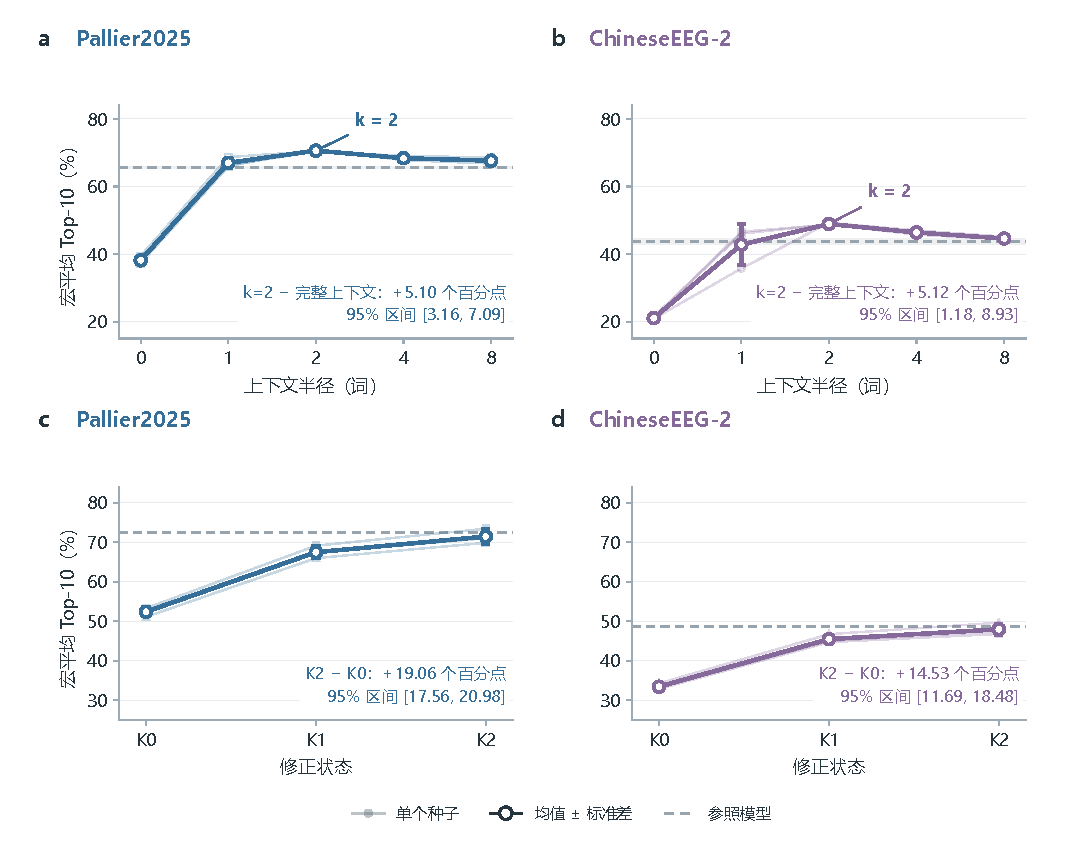
\includegraphics[width=\linewidth]{word_core_with_effects.pdf}
    \caption{词级检索结果（$50$ 词候选，宏平均 Top-$10$）。a,b：不同上下文半径，灰虚线及灰带为完整上下文均值 $\pm$ SD；c,d：共享滚动状态，灰虚线为独立 K2 均值。浅线为单个种子，粗线及误差棒为均值 $\pm$ SD。各面板标出核心差值及 $95\%$ 区间。}
    \label{fig:word_core_evidence}
\end{figure}
\FloatBarrier

\subsection{后续神经输入逐步改善同一目标}

同一目标从 K0 至 K2 的候选排序逐步改善（图~\ref{fig:word_core_evidence}c,d）。
在固定 $50$ 词候选集上，Pallier2025 和 ChineseEEG-2 的宏平均 Top-$10$ 分别提高 $19.06$ 和 $14.53$ 个百分点。
主要改善出现在第一个后续词窗到达之后，第二个后续词窗带来进一步增益；
共享模型的 K2 与单独训练的 K2 具有接近的预测表现，从而使同一组参数可覆盖三个可见状态。

延长单个目标词的观察窗口至 $1.28\,\mathrm{s}$ 或 $1.50\,\mathrm{s}$，并未达到当前跨词模型的词级检索水平（图~\ref{fig:word_controls}）。
该比较同时涉及历史词窗可见性与输入组织方式，因此仅用于说明延长单词输入不能直接替代当前局部上下文设置。
与仅输入目标词的半径 $0$ 模型相比，引入邻近词窗也具有明显的性能优势。

\begin{figure}[!htbp]
    \centering
    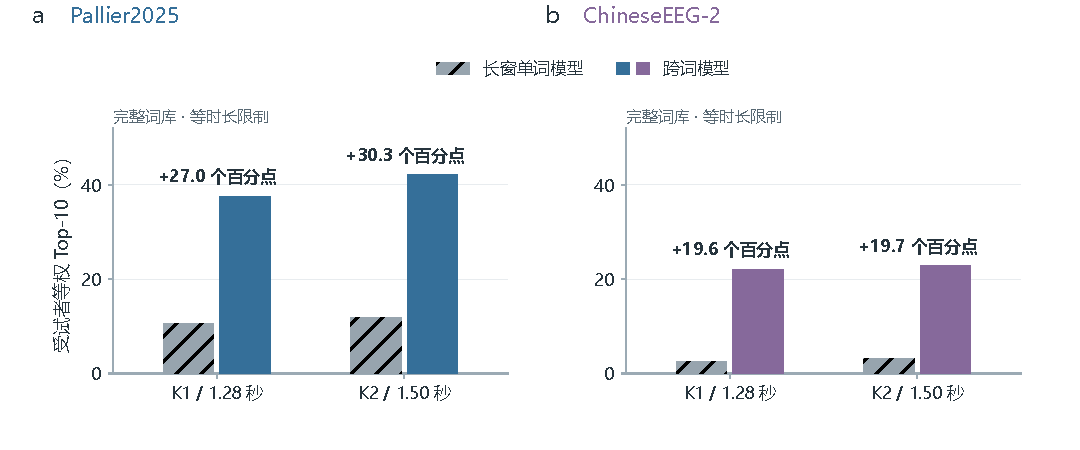
\includegraphics[width=\linewidth]{long_window_comparison.pdf}
    \caption{相近输入可用时刻下的长窗单词模型与局部跨词模型比较。a、b 分别对应 Pallier2025 与 ChineseEEG-2；使用完整训练词库下的受试者等权 Top-$10$。每对结果仅在对应跨词模型的最后输入词窗不晚于长窗结束的共同词位上计算，柱为三个种子的均值，标注为跨词模型减长窗模型的差值。}
    \label{fig:word_controls}
\end{figure}
\FloatBarrier

\subsection{滚动修正的文本收益与输入等待}

\paragraph{法语}
在 Pallier2025 上，滚动修正 C 使平均片段 BLEU-1 从 A 的 $8.37\%$ 提高至 $13.46\%$，
WER 由 $94.94\%$ 降至 $89.11\%$（表~\ref{tab:main}，图~\ref{fig:forest}）。
固定首次 K0 表示、仅重新搜索近期文本的 B，BLEU-1 为 $8.94\%$；
允许历史神经表示更新后，C 比 B 再提高约 $4.52$ 个百分点。
只允许一次回修的 C1 达到 $12.17\%$，平均额外输入等待为 $0.265\,\mathrm{s}$。
在当前序列搜索规则下，表示更新与有限回修能够带来较明确的文本收益。

\paragraph{中文}
ChineseEEG-2 的词级更新同样有效，但序列指标呈现不同结果。
A 到 C 的平均片段 BLEU-1 为 $9.25\%$ 至 $9.76\%$，增益 $+0.51$ 个百分点，
其配对区间 $[-0.41,1.42]$ 跨越零；WER 从 $97.54\%$ 降至 $95.97\%$，
词位准确率从 $2.31\%$ 升至 $3.98\%$。
固定 K0 的文本重搜 B 并未带来相同改善。
中文结果表明，词级候选排序的增益未必同步表现为 BLEU-1 的提高。
C 相对 A、B 的 WER 和词位准确率差异经双侧 Holm 校正后仍成立，具体数值见附录~\ref{sec:supp_statistics}。

\paragraph{与完整片段比较}
Pallier2025 的完整片段策略 F 获得最高 BLEU-1（$15.51\%$）。
在相同整段搜索条件下，F-local 沿用最终局部神经表示，BLEU-1 为 $13.72\%$，
接近 C 的 $13.46\%$；采用完整上下文模型的 F 带来进一步改善。
ChineseEEG-2 上，C、F-local 和 F 的 BLEU-1 差别较小。
C 相对首次预测平均增加 $0.502\,\mathrm{s}$（法语）和 $0.542\,\mathrm{s}$（中文）的输入等待，
比完整片段平均节省 $1.81\,\mathrm{s}$ 和 $1.51\,\mathrm{s}$（图~\ref{fig:tradeoff}）。

\begin{table}[!htbp]
    \centering
    \papertablestyle
    \caption{四种输出策略的平均片段 BLEU-1 与 WER（\%）。完整六策略结果见附录表~\ref{tab:sequence_complete_metrics}。}
    \label{tab:main}
    \label{tab:sentence_revision_full}
    % Presentation only: canonical manuscript_text_stage3_v1 exports.
\begingroup
\papertablestyle
\begin{tabular}{@{}lrrrr@{}}
\toprule
策略 & \multicolumn{2}{c}{Pallier2025} & \multicolumn{2}{c}{ChineseEEG-2} \\
\cmidrule(lr){2-3}\cmidrule(lr){4-5}
 & BLEU-1 $\uparrow$ & WER $\downarrow$ & BLEU-1 $\uparrow$ & WER $\downarrow$ \\
\midrule
A 固定输出 & 8.37 & 94.94 & 9.25 & 97.54 \\
C1 一次回修 & 12.17 & 90.58 & 9.74 & 97.00 \\
C 滚动修正 & 13.46 & 89.11 & 9.76 & 95.97 \\
F 完整片段 & 15.51 & 88.21 & 9.96 & 96.10 \\
\bottomrule
\end{tabular}
\endgroup

\end{table}

\begin{figure}[!htbp]
    \centering
    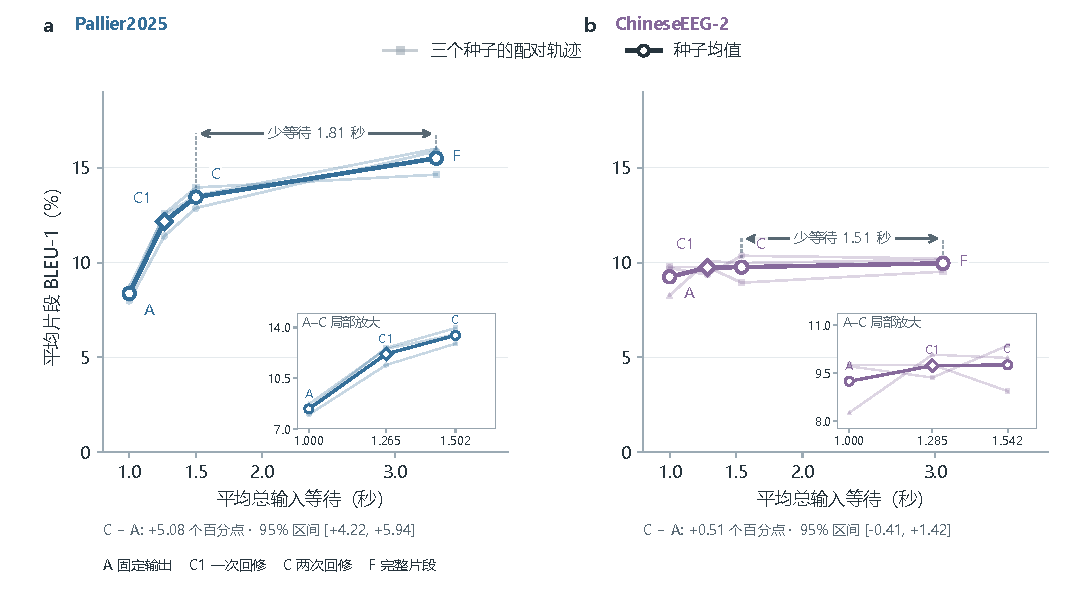
\includegraphics[width=\linewidth]{quality_wait_ac1cf_v2_test.pdf}
    \caption{文本质量与平均总输入等待。浅线为单个种子，空心点为种子均值；插图放大 A/C1/C。箭头为 C 相对 F 的等待节省。总等待包含自身 $1\,\mathrm{s}$ 神经窗。}
    \label{fig:tradeoff}
    \label{fig:sentence_full_context_tradeoff}
\end{figure}

\begin{figure}[!htbp]
    \centering
    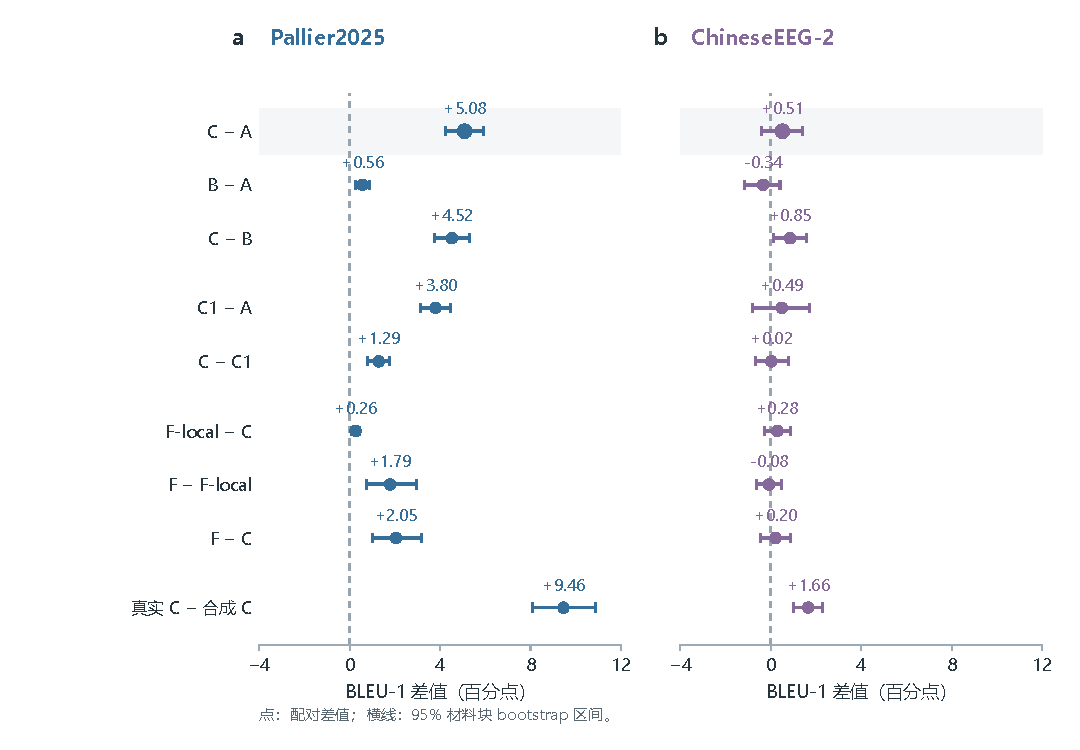
\includegraphics[width=\linewidth]{sequence_effects_forest.pdf}
    \caption{文本策略间的平均片段 BLEU-1 配对差值（百分点）。点为差值，横线为点态 $95\%$ 材料块 bootstrap 区间，虚线表示零；不将点态区间直接解释为多重比较校正后的检验结论。}
    \label{fig:forest}
\end{figure}
\FloatBarrier

\subsection{回修收益与输出稳定性}

从最终词位结果看，回修的净效果为正，改错为对的词位多于改对为错。
但逐次观察时，约 $88$--$94\%$ 的改写发生在错误词之间，最终词位恢复与输出稳定性需要分别评价（图~\ref{fig:sentence_display_edit_composition}；案例见附录图~\ref{fig:sentence_examples_full}）。


\begin{figure}[!htbp]
    \centering
    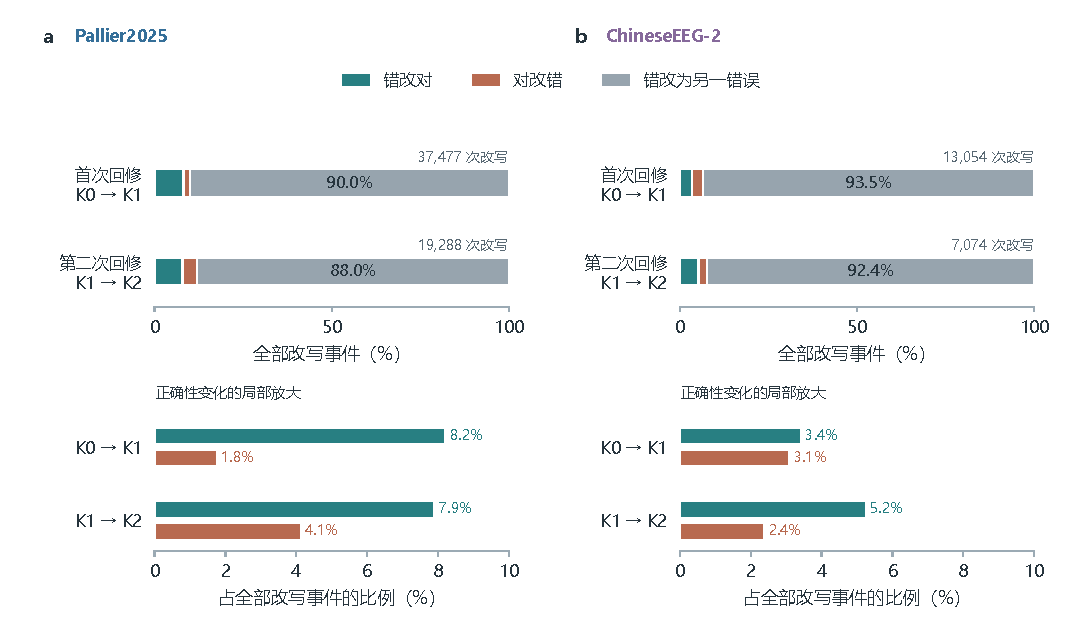
\includegraphics[width=\linewidth]{13_display_edit_composition.pdf}
    \caption{回修事件类型。仅统计输出发生变化的事件，合并三个种子；上排为三类改写组成，下排放大错改对和对改错的比例。}
    \label{fig:sentence_display_edit_composition}
\end{figure}
\FloatBarrier

\section{讨论}

\subsection{神经上下文的局部性}

在两个数据集上，少量邻近词窗已经能够带来较大的候选排序改善，继续扩大上下文范围并未持续提高主指标。
在固定 $50$ 词候选集上，局部范围对宏平均 Top-$10$ 更有利，而完整训练词库下的 Top-$1$ 不呈现一致优势，
说明不同评价尺度对上下文范围的响应存在差异。
长窗单词模型未达到当前局部跨词模型的检索水平，但这并不构成对跨词神经信息来源的单独识别。
本文更关注有限上下文在既定输入与模型协议下的实用表现，以及随后可实现的质量—等待折中。

\subsection{词级与序列级结果的差异}
\label{sec:discussion_word_sentence}

局部窗口在词级宏平均 Top-$10$ 上占优，而在法语 MEG 的最终文本质量比较中，完整片段策略 F 获得更高的 BLEU-1。
宏平均检索对词类型等权，文本指标则同时受到词频、候选构造和序列搜索规则影响，两者不对应相同的优化目标。
法语的 F-local 与 C 的最终文本质量接近，使用完整上下文模型的策略 F 进一步提高 BLEU-1；
F 和 F-local 来自不同上下文范围下独立训练的模型。
中文 EEG 各策略的文本差异较小。
上述实验用于比较不同输入等待与搜索协议下的预测表现，不将数据集之间的差异归因为单一神经或语言机制。

\subsection{滚动修正与输出稳定性}

多数回修仍发生在错误词之间，输出稳定性需要与最终文本质量分别评价。
后续工作可根据候选得分边际或置信度触发回修，并采用重翻译研究中的归一化擦除指标评价显示稳定性\cite{arivazhagan2020retranslation}。

\subsection{局限}

本文仍有若干适用边界。
首先，实验基于已知词级起始时刻、片段边界和目标词数的离线顺序重放，
输入等待仅反映神经窗口可用时刻，不包含模型推断与文本搜索耗时。
其次，相邻词窗高度重叠，模型性能可能受到词间时间间隔及其他输入结构线索的影响；
本文不对这些线索与词相关脑活动的贡献作定量分离。
再次，测试受试者出现在训练阶段，因此当前结果反映已见受试者上的新材料表现，文本绝对词位恢复率也仍然有限。
最后，两个数据集均来自《小王子》，语言模型可能在预训练阶段接触相关文本；
本文不将最终文本得分解释为神经信息贡献的独立估计。

\section{结论}

本文研究已知词级对齐条件下非侵入式语言解码的有限等待与滚动预测修正。
通过比较局部词窗与完整上下文模型，我们发现两个自然连续聆听数据集上的局部上下文能够在固定候选词级检索中取得良好表现。
在此基础上，共享滚动模型允许目标词在自身神经窗可用后先行预测，
再利用最多两个后续词窗更新近期预测，从而形成初判、回修与最终固定的连续输出过程。

在现有序列解码协议下，法语 MEG 的滚动修正改善了最终文本质量，中文 EEG 的收益主要体现于 WER 和词位准确率；
有限回修同时带来了可量化的输入等待与输出改写代价。
本文的结论限于已知词级对齐的离线重放设置。
未来可考虑将有限等待和历史预测修正推广到无精确事件对齐的 CTC 类连续神经解码框架；
在连续输入下限制未来帧可见范围，进一步评估预测质量、等待和输出稳定性。

\FloatBarrier
\bibliographystyle{IEEEtran}
\bibliography{../references/references}

\clearpage
\appendix
\setcounter{figure}{0}
\setcounter{table}{0}
\makeatletter
\@addtoreset{figure}{section}
\@addtoreset{table}{section}
\makeatother
\renewcommand{\thefigure}{\thesection\arabic{figure}}
\renewcommand{\thetable}{\thesection\arabic{table}}
\renewcommand{\theHfigure}{appendix.\thesection.\arabic{figure}}
\renewcommand{\theHtable}{appendix.\thesection.\arabic{table}}
% !TeX root = main.tex

\section{实现细节}
\label{sec:supp_settings}

\subsection{数据与词库}

表~\ref{tab:test_population} 汇总两个数据集的词库规模、候选数、训练词库覆盖率和测试范围。
训练词库只包含训练材料中的词。
验证选模时，从 $50$ 词候选中移除验证集未出现的词；测试时保留全部 $50$ 个候选。
ChineseEEG-2 依据实际朗读标点形成片段：在强标点处结束，弱标点后达到 $16$ 词时优先切分，
并将片段限制为最多 $32$ 词或 $15\,\mathrm{s}$，记录末尾保留剩余词位。

\begin{table}[htbp]
    \centering
    \papertablestyle
    \caption{词库、候选数及测试评价范围。查询数、片段数和词位数按一次模型评价计。}
    \label{tab:test_population}
    % Presentation only: simplify_appendix_tables_test_v2.py; verified frozen sources.
\begingroup
\papertablestyle
\begin{tabular}{@{}lrr@{}}
\toprule
项目 & Pallier2025 & ChineseEEG-2 \\
\midrule
训练词库 & 2020 & 2180 \\
训练词库覆盖率 & 82.49\% & 84.53\% \\
验证选模候选：词模型 & 50 & 47 \\
验证选模候选：上下文模型 & 49 & 46 \\
测试词检索候选 & 50 & 50 \\
\addlinespace
局部范围测试查询 & 8930 & 3444 \\
可见状态共同查询 & 7440 & 2872 \\
序列测试片段 & 1940 & 808 \\
序列参考词位 & 18450 & 8480 \\
序列材料块 & 39 & 21 \\
\bottomrule
\end{tabular}
\endgroup

\end{table}

文本表示由冻结的 BGE-M3 编码器得到。
每个词单独编码，取末层首个 token 的隐藏状态并做 $L_2$ 归一化：
\[
\mathbf y_i=\mathbf h_{i,\mathrm{first}}^{(L)}\big/\|\mathbf h_{i,\mathrm{first}}^{(L)}\|_2 .
\]


\subsection{模型与训练}
\label{sec:supp_model_training}

神经信号重采样至 $50$~Hz，主实验的 $1\,\mathrm{s}$ 词窗包含 $50$ 个时间点。
长窗对照分别使用 $64$ 和 $75$ 个时间点，对应 $1.28$ 和 $1.50\,\mathrm{s}$；
长窗词模型从头训练，沿用原词模型的训练配置和验证选模规则。
上下文 Transformer 为 $16$ 层、$16$ 个注意力头，隐藏维度 $1024$，
注意力 dropout 为 $0.1$，前馈层不使用 dropout。

词模型从头训练。
上下文模型加载同种子词模型的最佳检查点，新建上下文网络；
第一轮冻结神经编码器，之后联合训练。
两个阶段均使用 SigLIP 对比损失\cite{zhai2023siglip} 和 AdamW 优化器，
学习率 $10^{-4}$，余弦退火，批次大小 $128$，权重衰减 $0$，FP16 混合精度。
每阶段最多 $30$ 轮，验证指标连续 $10$ 轮未改善即停止。
检查点按验证集宏平均 Top-$10$ 选择：
词模型使用全部合格查询，上下文模型使用共同词位，共享滚动模型按 K2 选模。
各条件的输入和监督范围见表~\ref{tab:model_settings}。

\begin{table}[htbp]
    \centering
    \papertablestyle
    \caption{各模型的输入与训练设置。范围相对于目标词给出。独立 K2 与局部半径 $2$ 的输入和监督相同，使用同一个检查点。}
    \label{tab:model_settings}
    % Presentation only: simplify_appendix_tables_test_v2.py; verified frozen sources.
\begingroup
\papertablestyle
\begin{tabular}{@{}llll@{}}
\toprule
模型 & 输入范围 & 训练目标 & 参数关系 \\
\midrule
词模型 & 目标词神经窗 & 单词映射 & 不含上下文网络 \\
局部窗口 & $[-k,k]$ & 各词每轮一次 & 各半径分别训练 \\
完整上下文 & 片段内全部词 & 各词每轮一次 & 单独训练 \\
独立可见状态 & $[-2,r]$ & 各词每轮一次 & 各状态分别训练 \\
共享滚动模型 & $[-2,r]$ & \shortstack[l]{遍历到达时刻\\监督 K0/K1/K2} & 三个状态共享参数 \\
\bottomrule
\end{tabular}
\endgroup

\end{table}


\subsection{文本序列解码}
\label{sec:supp_sentence_settings}

语言模型对每个前缀生成若干条续写，每条只取第一个完整词作为候选，并去除重复。
两个数据集均使用连续叙述提示，提示中不包含刺激书名或内容：
法语为“Écrivez un paragraphe de récit en français. Donnez seulement le texte, sans titre ni liste.”；
中文为“请用中文写一段连续的叙述文字。只给出正文，不要标题或列表。”
提示后接两个换行，再拼接已解码前缀。

法语通常以空格连接词，但省音前项（如 c、j、l、d、qu）与后词之间插入撇号，
例如将 c 和 est 还原为 \textit{c'est}；以连字符开头的词直接接到前词。
中文词序列直接拼接，不插入空格。
前缀和加入候选后的文本分别整串编码，语言分数为两条整串文本的对数概率之差；
若拼接改变了边界 token，旧、新文本均从共同 token 前缀后的部分计算。
这避免将独立词编码的 token 概率直接拼接。
神经相似度乘以固定系数后，在训练词库和本步新提出的词库外候选上做 softmax。

语言权重使用验证材料上的种子 $0$、策略 A 的 WER 选择，平局时取较小值。
法语和中文分别选得 $\lambda=0.1$ 与 $0.5$，
同一数据集的全部策略和训练种子沿用相同提示、权重和搜索配置。
所有文本结果均按上述配置重新解码。

\begin{table}[!htbp]
    \centering
    \papertablestyle
    \caption{文本序列解码参数。两个数据集的语言权重分别选择；其余参数相同。}
    \label{tab:sentence_decoder_settings}
    % Rendered only from verified manuscript_text_stage3_v1 exports.
% Presentation only: verified reports/exports; polish_main_assets_test_v2.py.
\begingroup
\papertablestyle
\begin{tabular}{@{}lll@{}}
\toprule
设置 & Pallier2025 & ChineseEEG-2 \\
\midrule
语言模型 & \multicolumn{2}{l}{Qwen2.5-1.5B 基础版} \\
神经检索候选／词位 & \multicolumn{2}{l}{20} \\
神经相似度缩放系数 & \multicolumn{2}{l}{10} \\
束搜索保留序列数 & \multicolumn{2}{l}{5} \\
每个前缀的候选续写数 & \multicolumn{2}{l}{5} \\
每条续写的最大新 token 数 & \multicolumn{2}{l}{16} \\
近期重搜词位数（B/C） & \multicolumn{2}{l}{3} \\
语言模型上下文上限 & \multicolumn{2}{l}{32768 token} \\
验证语言权重候选 & \multicolumn{2}{l}{0, 0.025, 0.1, 0.5, 1.5} \\
语言权重选模指标 & \multicolumn{2}{l}{验证材料策略 A 的 WER} \\
权重平局规则 & \multicolumn{2}{l}{取较小值} \\
\midrule
测试固定语言权重 & 0.1 & 0.5 \\
\bottomrule
\end{tabular}
\endgroup

\end{table}

平均片段 BLEU-1 先在每个片段计算，再依次在受试者内、受试者间和种子间平均。
WER 和词位准确率按词位汇总，再对训练种子平均。

\subsection{统计方法}
\label{sec:statistics}
\label{sec:supp_statistics}

同一刺激在不同受试者中的呈现归为同一材料单元，每 $5$ 个连续材料单元构成一块，
在记录或章节内分层有放回抽样 $10000$ 次，取百分位数构造 $95\%$ 材料块 bootstrap 区间。
每次抽样对所有受试者、训练种子和比较条件使用相同的材料块，训练种子不另行重采样。
显著性检验采用双侧配对材料块符号翻转，使用 $1000000$ 次 Monte Carlo 抽样，
并按研究问题分组进行 Holm 多重比较校正；中文的 $21$ 个块另以全部 $2097152$ 种符号组合复核。
区间为点态区间，Holm 校正用于检验，不改变区间构造。
图中误差棒为三个训练种子的样本标准差。

\noindent\begin{minipage}{\linewidth}
ChineseEEG-2 中，
C$-$A 的 WER 差值为 $-1.57$ $[-2.07,-1.00]$ 个百分点，校正 $p=7.26\times10^{-4}$；词位准确率差值为 $+1.67$ $[1.07,2.19]$ 个百分点，校正 $p=7.26\times10^{-4}$。
C$-$B 的 WER 差值为 $-2.00$ $[-2.50,-1.48]$ 个百分点，校正 $p=4.80\times10^{-5}$；词位准确率差值为 $+2.08$ $[1.54,2.59]$ 个百分点，校正 $p=2.70\times10^{-5}$。
C$-$A 在两个数据集的三项文本指标组成的 $6$ 项比较内校正，
C$-$B 与 B$-$A 在两个数据集的三项指标组成的 $12$ 项比较内校正。
\end{minipage}

\clearpage
\section{完整词检索结果}
\label{sec:supp_word_statistics}

表~\ref{tab:word_complete_results} 给出 $50$ 词候选下全部模型的四项指标。
“全部”指真实词属于候选集合的全部合格查询，
“共同”进一步要求目标之后至少还有两个同片段词。
宏平均只在查询中实际出现的真实词类型上计算；
bootstrap 时按每次抽样实际出现的类型计算，两个比较条件使用相同的类型集合。

% Presentation only: formal test exports; consolidate_results_tables_test_v2.py.
\begingroup
\papertablestyle
\begin{longtable}{@{}lllrrrr@{}}
\caption{两个数据集的完整 $50$ 词候选检索结果（\%，三个种子均值 $\pm$ 样本标准差）。全部与共同查询分别列出；独立 K2 与局部半径 $2$ 共享检查点，比较时使用其共同查询行。}
\label{tab:word_complete_results}\label{tab:word_complete_pallier}\label{tab:word_complete_chinese}\\
\toprule
数据集 & 输入/模型 & 查询 & \shortstack{宏平均\\Top-$10$} & \shortstack{宏平均\\Top-$1$} & \shortstack{微平均\\Top-$10$} & \shortstack{微平均\\Top-$1$} \\
\midrule
\endfirsthead
\multicolumn{7}{l}{表~\ref{tab:word_complete_results}（续）}\\
\toprule
数据集 & 输入/模型 & 查询 & \shortstack{宏平均\\Top-$10$} & \shortstack{宏平均\\Top-$1$} & \shortstack{微平均\\Top-$10$} & \shortstack{微平均\\Top-$1$} \\
\midrule
\endhead
\midrule\multicolumn{7}{r}{续下页}\\\endfoot
\bottomrule\endlastfoot
Pallier2025 & 完整上下文 & 全部 & $65.52\pm0.31$ & $20.44\pm0.52$ & $68.53\pm0.78$ & $25.19\pm0.99$ \\
 &  & 共同 & $67.42\pm0.14$ & $21.23\pm0.47$ & $68.17\pm0.72$ & $24.66\pm1.04$ \\
\addlinespace
Pallier2025 & 局部半径 0 & 全部 & $38.16\pm1.15$ & $6.18\pm0.36$ & $36.91\pm0.97$ & $7.64\pm0.11$ \\
 &  & 共同 & $38.44\pm0.92$ & $6.15\pm0.24$ & $36.43\pm0.86$ & $7.22\pm0.06$ \\
\addlinespace
Pallier2025 & 局部半径 1 & 全部 & $67.00\pm1.50$ & $17.55\pm0.16$ & $67.18\pm1.47$ & $20.33\pm0.23$ \\
 &  & 共同 & $68.02\pm1.57$ & $17.59\pm0.25$ & $66.63\pm1.31$ & $19.26\pm0.22$ \\
\addlinespace
Pallier2025 & 局部半径 2 & 全部 & $70.62\pm0.34$ & $23.27\pm0.54$ & $72.95\pm0.23$ & $26.01\pm0.18$ \\
 &  & 共同 & $72.49\pm0.59$ & $23.55\pm0.55$ & $72.57\pm0.61$ & $24.86\pm0.37$ \\
\addlinespace
Pallier2025 & 局部半径 4 & 全部 & $68.38\pm0.63$ & $22.55\pm0.61$ & $71.02\pm1.33$ & $25.76\pm1.05$ \\
 &  & 共同 & $70.24\pm0.75$ & $23.17\pm0.91$ & $70.77\pm1.29$ & $25.09\pm0.80$ \\
\addlinespace
Pallier2025 & 局部半径 8 & 全部 & $67.64\pm0.91$ & $21.63\pm1.96$ & $70.35\pm1.17$ & $24.86\pm1.99$ \\
 &  & 共同 & $69.63\pm1.09$ & $22.46\pm1.95$ & $70.01\pm1.29$ & $24.35\pm1.72$ \\
\addlinespace
Pallier2025 & 独立 K0 & 全部 & $49.46\pm1.39$ & $9.64\pm0.44$ & $48.56\pm1.62$ & $11.58\pm0.81$ \\
 &  & 共同 & $49.60\pm1.47$ & $9.45\pm0.70$ & $48.15\pm1.61$ & $11.22\pm0.92$ \\
\addlinespace
Pallier2025 & 独立 K1 & 全部 & $68.29\pm1.08$ & $20.13\pm1.00$ & $69.49\pm1.41$ & $22.81\pm1.27$ \\
 &  & 共同 & $69.18\pm1.29$ & $20.42\pm1.05$ & $68.69\pm1.55$ & $21.88\pm1.10$ \\
\addlinespace
Pallier2025 & 共享 K0 & 全部 & $51.72\pm1.03$ & $11.23\pm0.59$ & $51.60\pm0.73$ & $13.43\pm0.31$ \\
 &  & 共同 & $52.35\pm1.15$ & $11.30\pm0.59$ & $51.10\pm0.71$ & $12.76\pm0.33$ \\
\addlinespace
Pallier2025 & 共享 K1 & 全部 & $66.05\pm1.55$ & $18.65\pm0.83$ & $67.38\pm1.21$ & $21.35\pm0.86$ \\
 &  & 共同 & $67.44\pm1.58$ & $19.44\pm0.80$ & $66.91\pm1.20$ & $20.81\pm0.86$ \\
\addlinespace
Pallier2025 & 共享 K2 & 全部 & $69.56\pm1.62$ & $21.77\pm1.26$ & $71.10\pm1.45$ & $24.32\pm1.11$ \\
 &  & 共同 & $71.41\pm1.82$ & $23.02\pm1.36$ & $71.37\pm1.49$ & $24.37\pm1.20$ \\
\addlinespace
\midrule
ChineseEEG-2 & 完整上下文 & 全部 & $43.79\pm0.86$ & $8.13\pm0.54$ & $47.96\pm0.20$ & $11.99\pm0.38$ \\
 &  & 共同 & $42.13\pm1.03$ & $8.10\pm0.67$ & $45.74\pm0.51$ & $11.30\pm0.77$ \\
\addlinespace
ChineseEEG-2 & 局部半径 0 & 全部 & $21.05\pm0.36$ & $1.37\pm0.27$ & $28.45\pm0.54$ & $3.12\pm1.34$ \\
 &  & 共同 & $21.88\pm0.76$ & $1.37\pm0.22$ & $28.49\pm0.95$ & $3.02\pm1.04$ \\
\addlinespace
ChineseEEG-2 & 局部半径 1 & 全部 & $42.78\pm6.12$ & $7.25\pm2.10$ & $46.86\pm4.48$ & $8.58\pm2.19$ \\
 &  & 共同 & $41.87\pm5.71$ & $7.16\pm1.98$ & $45.81\pm3.66$ & $8.73\pm1.97$ \\
\addlinespace
ChineseEEG-2 & 局部半径 2 & 全部 & $48.91\pm0.30$ & $9.35\pm0.64$ & $52.10\pm0.38$ & $10.60\pm0.90$ \\
 &  & 共同 & $48.62\pm0.07$ & $9.16\pm0.60$ & $50.53\pm1.20$ & $10.41\pm0.95$ \\
\addlinespace
ChineseEEG-2 & 局部半径 4 & 全部 & $46.39\pm0.64$ & $9.42\pm0.55$ & $52.61\pm0.95$ & $14.02\pm0.81$ \\
 &  & 共同 & $45.89\pm0.77$ & $9.49\pm0.45$ & $51.35\pm0.98$ & $13.50\pm0.51$ \\
\addlinespace
ChineseEEG-2 & 局部半径 8 & 全部 & $44.60\pm0.49$ & $8.79\pm0.12$ & $49.32\pm1.91$ & $12.36\pm0.57$ \\
 &  & 共同 & $43.05\pm0.94$ & $8.61\pm0.44$ & $47.05\pm1.97$ & $11.23\pm0.85$ \\
\addlinespace
ChineseEEG-2 & 独立 K0 & 全部 & $30.03\pm3.82$ & $2.95\pm0.45$ & $35.23\pm2.58$ & $5.77\pm1.55$ \\
 &  & 共同 & $30.07\pm3.51$ & $2.75\pm0.31$ & $35.49\pm2.06$ & $6.55\pm1.97$ \\
\addlinespace
ChineseEEG-2 & 独立 K1 & 全部 & $46.19\pm0.93$ & $9.32\pm0.15$ & $49.18\pm1.83$ & $9.10\pm0.70$ \\
 &  & 共同 & $45.44\pm0.63$ & $8.92\pm0.31$ & $48.35\pm1.92$ & $8.96\pm1.10$ \\
\addlinespace
ChineseEEG-2 & 共享 K0 & 全部 & $33.96\pm0.93$ & $4.21\pm0.34$ & $39.14\pm1.26$ & $5.63\pm2.48$ \\
 &  & 共同 & $33.40\pm0.73$ & $3.72\pm0.51$ & $39.16\pm1.57$ & $6.09\pm2.69$ \\
\addlinespace
ChineseEEG-2 & 共享 K1 & 全部 & $44.60\pm1.03$ & $8.11\pm0.46$ & $48.38\pm2.00$ & $9.20\pm1.90$ \\
 &  & 共同 & $45.44\pm1.09$ & $8.47\pm0.27$ & $49.56\pm2.00$ & $9.77\pm1.97$ \\
\addlinespace
ChineseEEG-2 & 共享 K2 & 全部 & $46.83\pm1.58$ & $9.05\pm0.31$ & $49.54\pm2.04$ & $10.84\pm0.87$ \\
 &  & 共同 & $47.93\pm1.49$ & $9.50\pm0.41$ & $50.94\pm2.08$ & $11.73\pm0.80$ \\
\addlinespace
\end{longtable}
\endgroup


共享模型与独立模型的比较见表~\ref{tab:word_complete_results} 的共同查询行；独立 K2 对应局部半径 $2$。


\begin{table}[!htbp]
    \centering
    \papertablestyle
    \caption{完整训练词库下局部与完整上下文的词检索结果（\%）。词库外目标计为未命中，差值为局部减完整上下文。}
    \label{tab:full_vocab_comparison}
    % Presentation only: verified reports/exports; polish_main_assets_test_v2.py.
\begingroup
\papertablestyle
\begin{tabular}{@{}llrrrl@{}}
\toprule
数据集 & 指标 & 局部 $k=2$ & 完整上下文 & 差值 (pp) & $95\%$ CI (pp) \\
\midrule
Pallier2025 & Macro Top-$10$ & 8.45 & 7.27 & $+1.18$ & $[0.63, 1.85]$ \\
 & Micro Top-$10$ & 29.46 & 27.30 & $+2.16$ & $[1.11, 3.15]$ \\
\addlinespace
 & Macro Top-$1$ & 2.45 & 2.17 & $+0.28$ & $[-0.02, 0.56]$ \\
 & Micro Top-$1$ & 11.12 & 11.33 & $-0.21$ & $[-1.13, 0.66]$ \\
\midrule
ChineseEEG-2 & Macro Top-$10$ & 4.84 & 3.50 & $+1.33$ & $[1.05, 2.01]$ \\
 & Micro Top-$10$ & 15.02 & 13.19 & $+1.83$ & $[0.75, 3.04]$ \\
\addlinespace
 & Macro Top-$1$ & 0.83 & 0.72 & $+0.11$ & $[-0.25, 0.37]$ \\
 & Micro Top-$1$ & 3.42 & 4.54 & $-1.13$ & $[-1.95, -0.33]$ \\
\bottomrule
\end{tabular}
\endgroup

\end{table}

\FloatBarrier
\clearpage
\section{文本序列补充结果}
\label{sec:supp_sentence}

表~\ref{tab:sentence_by_seed_acf} 报告逐种子结果，
表~\ref{tab:sequence_complete_metrics} 汇总全部六种策略。
图~\ref{fig:sentence_participant_gains} 展示受试者收益，
表~\ref{tab:input_wait_complete} 报告输入等待分布。

% Rendered only from verified manuscript_text_stage3_v1 exports.
\begingroup
\papertablestyle
\begin{longtable}{@{}llrrrr@{}}
\caption{六种策略的逐种子结果（\%）。各策略使用相同的语言提示与前缀格式；F-local 使用与 C 相同的最终局部表示。}
\label{tab:sentence_by_seed_acf}\\
\toprule
数据集 & 策略 & 种子 & BLEU-1 $\uparrow$ & WER $\downarrow$ & \shortstack{词位\\准确率 $\uparrow$} \\
\midrule\endfirsthead
\multicolumn{6}{l}{表~\ref{tab:sentence_by_seed_acf}（续）}\\
\toprule
数据集 & 策略 & 种子 & BLEU-1 $\uparrow$ & WER $\downarrow$ & \shortstack{词位\\准确率 $\uparrow$} \\
\midrule\endhead
\midrule\multicolumn{6}{r}{续下页}\\\endfoot
\bottomrule\endlastfoot
Pallier2025 & A & 0 & 7.98 & 95.11 & 4.85 \\
 & B & 0 & 8.71 & 94.44 & 5.53 \\
 & C1 & 0 & 11.41 & 91.00 & 8.99 \\
 & C & 0 & 12.88 & 89.41 & 10.57 \\
 & F-local & 0 & 13.14 & 89.23 & 10.75 \\
 & F & 0 & 15.88 & 87.69 & 12.27 \\
\addlinespace
 & A & 1 & 8.43 & 94.85 & 5.09 \\
 & B & 1 & 9.13 & 94.14 & 5.82 \\
 & C1 & 1 & 12.58 & 90.18 & 9.77 \\
 & C & 1 & 13.96 & 88.48 & 11.50 \\
 & F-local & 1 & 14.31 & 88.14 & 11.81 \\
 & F & 1 & 14.64 & 88.85 & 11.12 \\
\addlinespace
 & A & 2 & 8.71 & 94.86 & 5.11 \\
 & B & 2 & 8.97 & 94.46 & 5.50 \\
 & C1 & 2 & 12.51 & 90.56 & 9.39 \\
 & C & 2 & 13.53 & 89.44 & 10.51 \\
 & F-local & 2 & 13.70 & 89.17 & 10.77 \\
 & F & 2 & 16.00 & 88.09 & 11.85 \\
\midrule
ChineseEEG-2 & A & 0 & 9.72 & 97.24 & 2.65 \\
 & B & 0 & 9.39 & 97.70 & 2.13 \\
 & C1 & 0 & 9.37 & 97.26 & 2.67 \\
 & C & 0 & 10.36 & 95.75 & 4.21 \\
 & F-local & 0 & 11.01 & 95.53 & 4.38 \\
 & F & 0 & 10.21 & 96.20 & 3.61 \\
\addlinespace
 & A & 1 & 9.77 & 97.02 & 2.76 \\
 & B & 1 & 9.42 & 97.70 & 2.21 \\
 & C1 & 1 & 9.77 & 96.70 & 3.20 \\
 & C & 1 & 8.94 & 96.17 & 3.76 \\
 & F-local & 1 & 9.51 & 95.91 & 4.02 \\
 & F & 1 & 9.53 & 96.23 & 3.69 \\
\addlinespace
 & A & 2 & 8.27 & 98.36 & 1.51 \\
 & B & 2 & 7.92 & 98.51 & 1.36 \\
 & C1 & 2 & 10.08 & 97.05 & 2.84 \\
 & C & 2 & 9.98 & 95.98 & 3.97 \\
 & F-local & 2 & 9.61 & 96.18 & 3.77 \\
 & F & 2 & 10.15 & 95.88 & 4.00 \\
\end{longtable}
\endgroup


\begin{table}[!htbp]
    \centering
    \papertablestyle
    \caption{六种策略的文本质量（\%）与平均总输入等待（s）。B 与 C 的输出固定时刻相同，F-local 与 F 相同。}
    \label{tab:sequence_complete_metrics}
    % Rendered only from verified manuscript_text_stage3_v1 exports.
% Presentation only: verified reports/exports; polish_main_assets_test_v2.py.
\begingroup
\papertablestyle
\begin{tabular}{@{}lrrrrrrrr@{}}
\toprule
策略 & \multicolumn{4}{c}{\textbf{Pallier2025}} & \multicolumn{4}{c}{\textbf{ChineseEEG-2}} \\
\cmidrule(lr){2-5}\cmidrule(lr){6-9}
 & \papertablehead{BLEU-1 $\uparrow$}{(\%)} & \papertablehead{WER $\downarrow$}{(\%)} & \shortstack{词位\\准确率 $\uparrow$\\(\%)} & \papertablehead{输入等待}{(s)} & \papertablehead{BLEU-1 $\uparrow$}{(\%)} & \papertablehead{WER $\downarrow$}{(\%)} & \shortstack{词位\\准确率 $\uparrow$\\(\%)} & \papertablehead{输入等待}{(s)} \\
\midrule
A 固定输出 & 8.37 & 94.94 & 5.02 & 1.000 & 9.25 & 97.54 & 2.31 & 1.000 \\
B 固定表示重搜 & 8.94 & 94.35 & 5.62 & 1.502 & 8.91 & 97.97 & 1.90 & 1.542 \\
\addlinespace
\textbf{C1 一次回修} & 12.17 & 90.58 & 9.38 & 1.265 & 9.74 & 97.00 & 2.90 & 1.285 \\
\textbf{C 滚动修正} & 13.46 & 89.11 & 10.86 & 1.502 & 9.76 & 95.97 & 3.98 & 1.542 \\
\addlinespace
F-local 局部整段 & 13.72 & 88.85 & 11.11 & 3.311 & 10.05 & 95.87 & 4.06 & 3.057 \\
F 完整片段 & 15.51 & 88.21 & 11.75 & 3.311 & 9.96 & 96.10 & 3.77 & 3.057 \\
\bottomrule
\end{tabular}
\endgroup

\end{table}

\begin{figure}[!htbp]
    \centering
    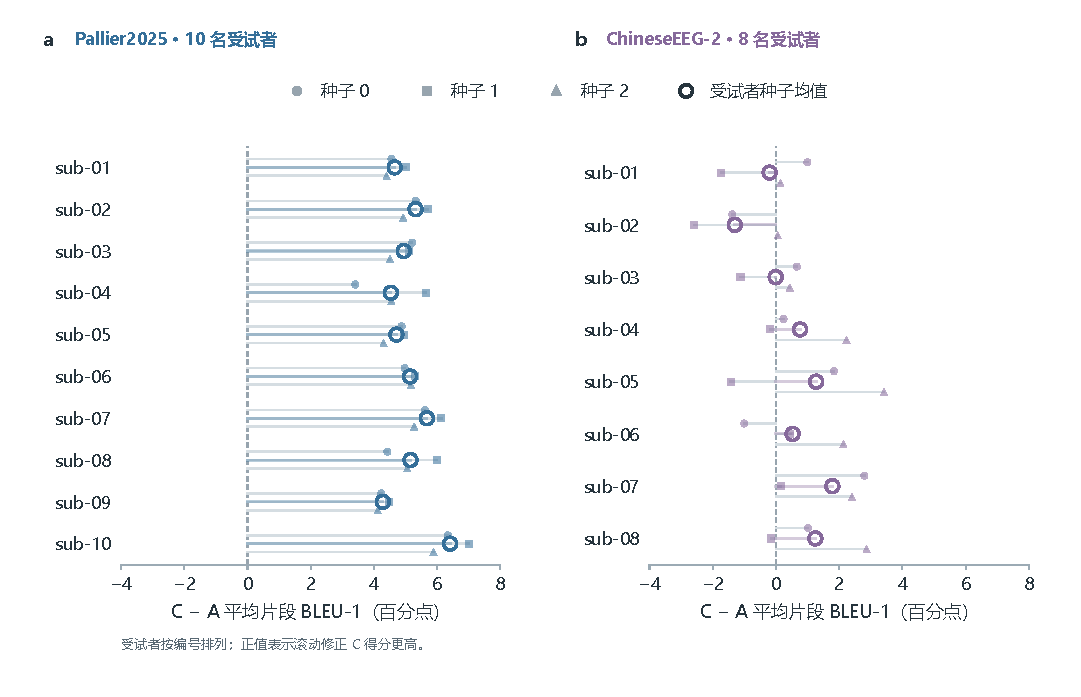
\includegraphics[width=\linewidth]{14_participant_gains.pdf}
    \caption{受试者层面 C 减 A 的平均片段 BLEU-1（百分点）。小符号为单个种子，空心圆为种子均值。ChineseEEG-2 的种子 $2$ 下 A 得分较低（$8.27\%$），种子 $1$ 的 C 减 A 为负。}
    \label{fig:sentence_participant_gains}
\end{figure}

\begin{table}[!htbp]
    \centering
    \papertablestyle
    \caption{全部测试词位的总输入等待（s）。等待从词起点计算，包含自身 $1\,\mathrm{s}$ 神经窗。}
    \label{tab:input_wait_complete}
    % Presentation only: simplify_appendix_tables_test_v2.py; verified frozen sources.
\begingroup
\papertablestyle
\begin{tabular}{@{}llrrrrr@{}}
\toprule
数据集 & 策略 & 词位数 & 均值 (s) & 中位 (s) & P90 (s) & \papertablehead{输入等待节省}{较 F (s)} \\
\midrule
Pallier2025 & A / K0 & 18450 & 1.000 & 1.000 & 1.000 & 2.311 \\
 & C / K2 & 18450 & 1.502 & 1.446 & 2.000 & 1.808 \\
 & F & 18450 & 3.311 & 2.342 & 6.670 & 0.000 \\
\addlinespace
ChineseEEG-2 & A / K0 & 8480 & 1.000 & 1.000 & 1.000 & 2.057 \\
 & C / K2 & 8480 & 1.542 & 1.480 & 2.120 & 1.514 \\
 & F & 8480 & 3.057 & 2.440 & 5.960 & 0.000 \\
\bottomrule
\end{tabular}
\endgroup

\end{table}

\begin{figure}[!htbp]
    \centering
    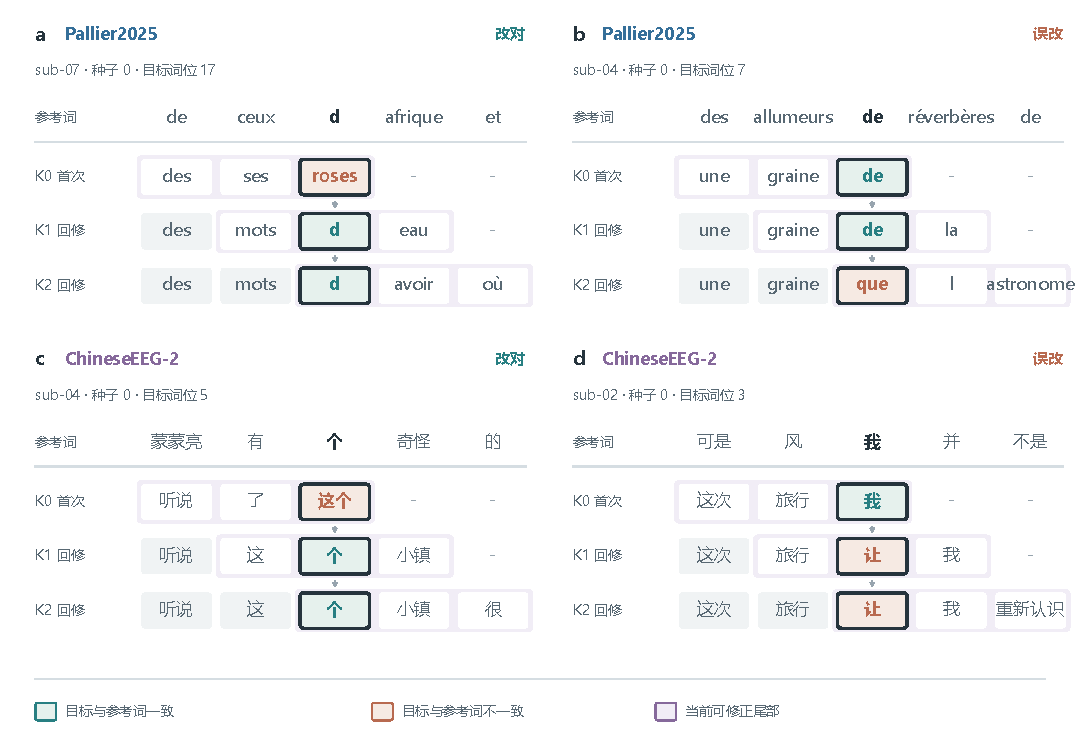
\includegraphics[width=\linewidth]{10_sentence_revision_examples.pdf}
    \caption{策略 C 的回修案例。三行依次为首次预测及两次回修；黑框标记目标词位，绿色和橙色分别表示与参考词一致和不一致。案例来自种子 $0$，各列对应固定词位。}
    \label{fig:sentence_examples_full}
\end{figure}

\FloatBarrier
\end{document}
